%!TEX root =  tfg.tex
\chapter{Dataset}

\begin{abstract}
The dataset is one of the most important things in an artificial inteligence project, we are going to define the dataset, how we obtained this data and the preprocessing methodology in order to increase the number of the data. 
\end{abstract}

\section[Dataset]{Dataset}
\subsection{Description}
In order to set the feasibility of the project we have to look for a good dataset which contains a great deal of different data. In our case it's not a hard task to acquire the data, the ISIC institute exposed in 2018 more than 20.000 skin lesion images during a challenge. 
\url{https://challenge2018.isic-archive.com/}

Furthermore exist other famous datasets like \emph{PH2Dataset} from the Oporto Universiy which the number of images is much lower but we can use some Data Augmentation techniques to improve the results.

\subsection{Acquisition of data}

The ISIC Archive contains over 23k images of skin lesions, labeled as 'benign' or 'malignant'. The first option to download the entire ISIC archive is via the direct download button on their website, which is the easiest and most comfortable way and doesn't always finish successfully for some reason. We suspect this is happening due to the large file size. 

\begin{figure}[H]
\centering
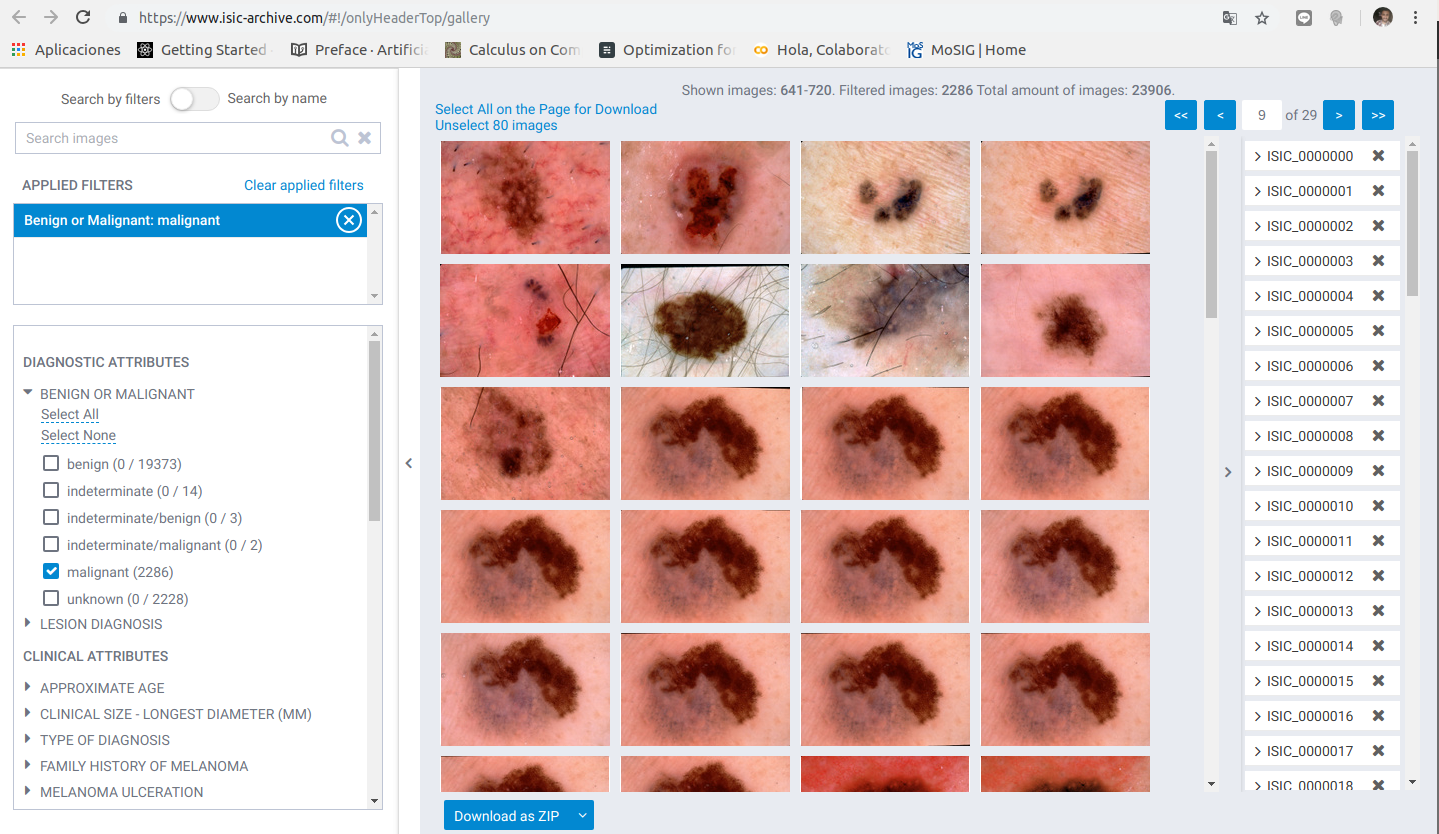
\includegraphics[width=0.8\textwidth]{./figures/isic-dataset}
\caption{Download the data from the ISIC website}
\end{figure}

The second option is to download the small partitions of the archive, called 'datasets' one by one. Seems rather good if you plan to download the archive only a few times and 

The third option is to download the archive using the Grider API provided in the website but seems unfeasible.


Thankfully, Oren Talmor and Gal Avineri have created a script which we can use to download all the ISIC archive easily \cite{isic-archive-downloader}. Furthermore we can filter and limit the number of images that we want to download.


After download the ISIC archive we divided in two separated folders:
\begin{itemize}
\item Trainning: The neuronal network will use the images in this folder to get trainning in every epochs.
\item Test: The neuronal network will use the images in this folder to validate the trainning process and calculate the accuracy of the model in every epochs.
\end{itemize}


\begin{figure}[H]
\centering
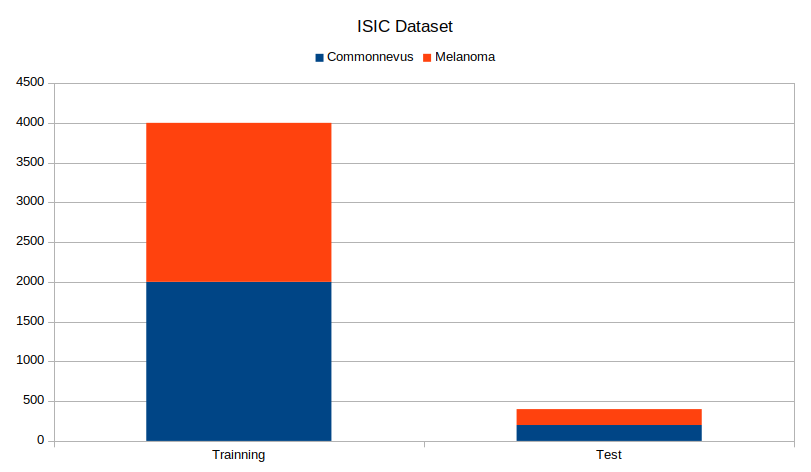
\includegraphics[width=0.8\textwidth]{./figures/dataset-plot-size}
\caption{Data divided in trainning and test groups}
\end{figure}

You can see in the figure that we divided the dataset in the two groups, 
4000 images will be used for trainning and 400 images for test porpouses.
Furthermore we have implemented some preprocessing techniques to increase the number of data but we will explain these techniques in the next section.

\subsection{Image preprocessing}
The image preprocessing is critical to subsequent steps and plays an important role in achieving a good performance. The source dermoscpic images provided by the competition are obtained from real clinic environment, which means that there are a great number of man-made interferences. The objective of preprocessing is to improve the quality of the source images,and make the following parts run easily.

\begin{figure}[H]
\centering
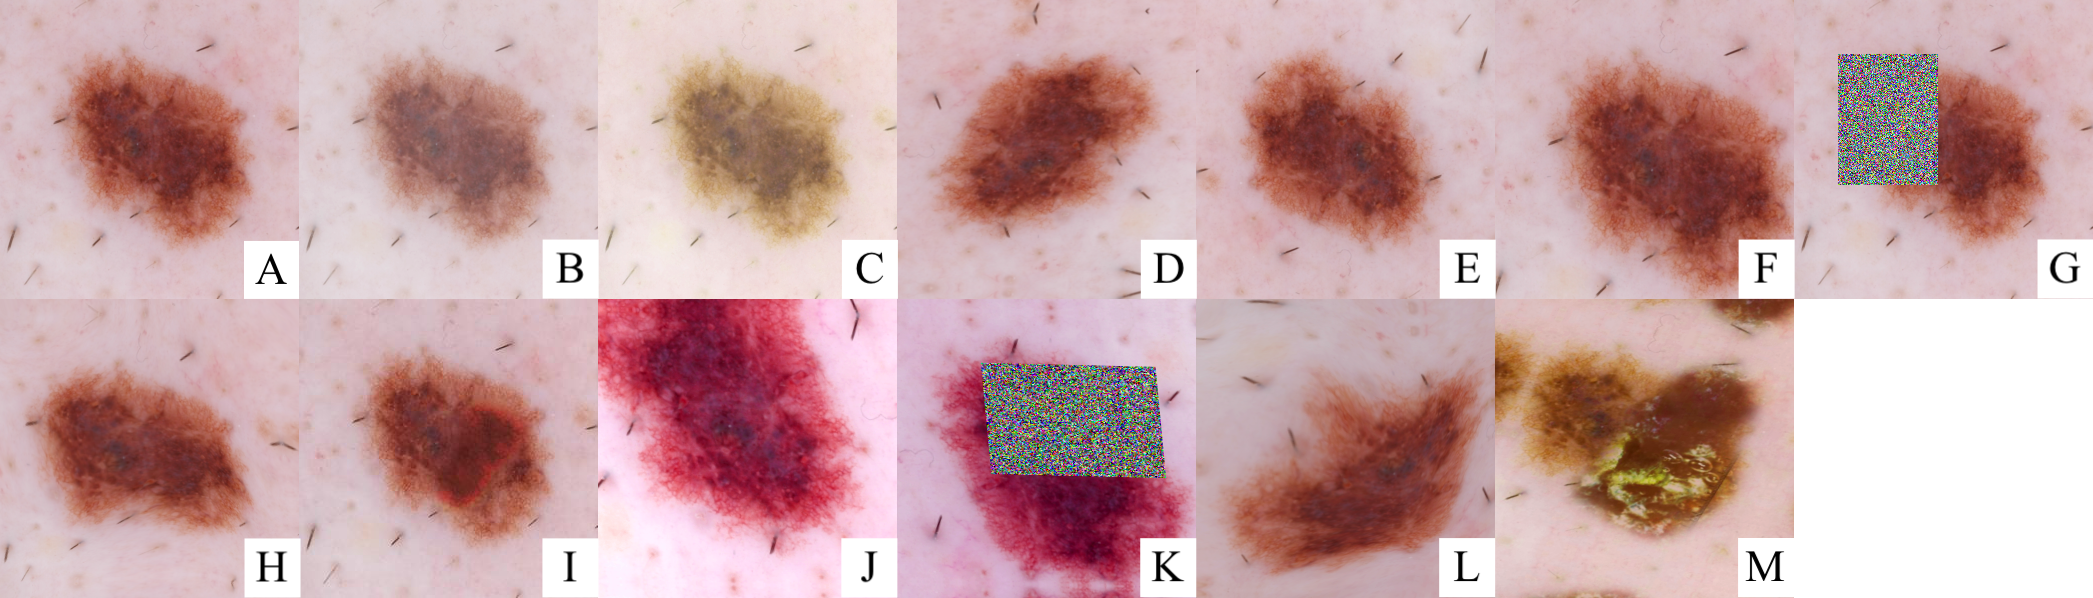
\includegraphics[width=0.8\textwidth]{./figures/data-augmentation}
\caption{Examples of data augmentation. \cite{data-augmentation-skin}}
\end{figure}

We are going to use some techniques for data augmentation. Data augmentation goal is to add new data
points to the input space by modifying training images while preserving semantic 
information and target labels \cite{data-augmentation-skin}. Thus, it is used to reduce overfitting. As we read from this paper, the results will increase if we use this techniques.


\begin{figure}[H]
\centering
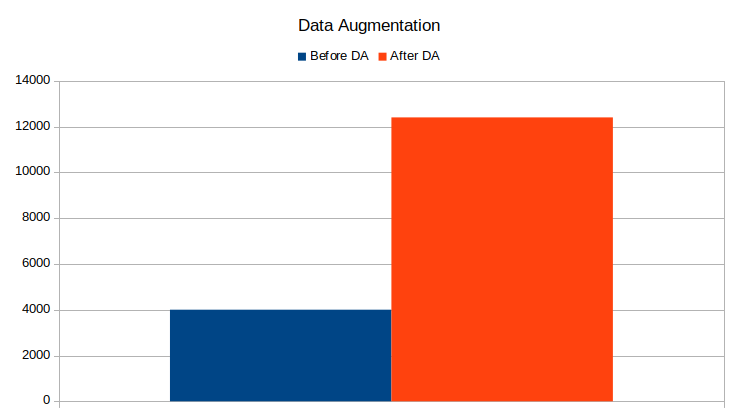
\includegraphics[width=0.8\textwidth]{./figures/data-augmentation-plot}
\caption{Number of data after apply data augmentation techniques}
\end{figure}

\chapter{Data analysis}

\begin{abstract}
What is the best architecture? Which parameters should we change? How do we define a good model? In this chapter we are going to explain all these questions, we are going to expose the 3 differents models that we are going to test and validate their results.

\end{abstract}

\section{Transfer Learning}
In practice, very few people train an entire Convolutional Network from scratch (with random initialization), because it is relatively rare to have a dataset of sufficient size. Instead, it is common to pretrain a ConvNet on a very large dataset (e.g. ImageNet, which contains 1.2 million images with 1000 categories), and then use the ConvNet either as an initialization or a fixed feature extractor for the task of interest.

Instead of random initializaion, we initialize the network with a pretrained network, like the one that is trained on imagenet 1000 dataset. We will freeze the weights for all of the network except that of the final fully connected layer. This last fully connected layer is replaced with a new one with random weights and only this layer is trained.

In the next tables we are going to define the models that we are going to train and test for our project.
\FloatBarrier
\begin{table*}[htb]
	\centering
	\begin{coolTable}{p{4cm}p{\textwidth-4.5cm}}{2}
{1º ResNet Model}
	\textbf{Architecture}&ResNet\\
	\textbf{Number of Layers}&18\\	
	\textbf{Optimizer}&Stochastic Gradient Descent\\
	\textbf{Learning rate}&0.001\\
	\textbf{Epochs}&11 \\
	\end{coolTable}
	\caption{Definition of the 1º model}
\end{table*}
\FloatBarrier

\newpage
\FloatBarrier
\begin{table*}[htb]
	\centering
	\begin{coolTable}{p{4cm}p{\textwidth-4.5cm}}{2}
{2º ResNet Model}
	\textbf{Architecture}&ResNet\\
	\textbf{Number of Layers}&50\\
	\textbf{Optimizer}&Stochastic Gradient Descent\\
	\textbf{Learning rate}&0.001\\
	\textbf{Epochs}&21 \\
	\end{coolTable}
	\caption{Definition of the 2º model}
\end{table*}
\FloatBarrier

\FloatBarrier
\begin{table*}[htb]
	\centering
	\begin{coolTable}{p{4cm}p{\textwidth-4.5cm}}{2}
{3º DenseNet Model}
	\textbf{Architecture}&Densenet\\
	\textbf{Number of Layers}&101\\	
	\textbf{Optimizer}&Stochastic Gradient Descent\\
	\textbf{Learning rate}&0.001\\
	\textbf{Epochs}&21 \\
	\end{coolTable}
	\caption{Definition of the 3º model}
\end{table*}
\FloatBarrier


\chapter{Software analysis}

\begin{abstract}
In this chapter we are going to define the requirements of our software solution. Furthermore, the risks and the initial costs of the project will be detailed.
\end{abstract}


\section{Requirements of the software}

The main goal of this project is research about Deep Learning and how can we use this techniques to analize skin cancer images, so we are not in the classical software lifecycle. However, we are going to provide an API that we will consume from an App to get the results of the predictions, this is just a prototype to show the power of this technology and how can we use in a real world.


\FloatBarrier
\begin{table*}[htb]
	\centering
	\begin{coolTable}{p{4cm}p{\textwidth-4.5cm}}{2}
{REQ-001: Obtain the dataset and divide it}
	\textbf{Version}&1.0\\
	\textbf{Author}&Álvaro González Jiménez\\
	\textbf{Description}&The system must have all the images available and divided in two categories (trainning and tests).\\
	\textbf{Priority}&High \\
	\textbf{Status}&Done\\
	\textbf{Comments}& - \\
	\end{coolTable}
	\caption{REQ-001 Obtain the dataset and divide it}
\end{table*}


\begin{table*}[htb]
	\centering
	\begin{coolTable}{p{4cm}p{\textwidth-4.5cm}}{2}
{REQ-002: Preprocessing dataset images}
	\textbf{Version}&1.0\\
	\textbf{Author}&Álvaro González Jiménez\\
	\textbf{Description}&The system must to provide a set of tools to increase the number of images in the dataset in order to get better results.\\
	\textbf{Priority}&High \\
	\textbf{Status}&Done\\
	\textbf{Comments}& - \\
	\end{coolTable}
	\caption{REQ-002 Preprocessing dataset images}
\end{table*}

\begin{table*}[htb]
	\centering
	\begin{coolTable}{p{4cm}p{\textwidth-4.5cm}}{2}
{REQ-003: Hyperparameter optimization or tuning}
	\textbf{Version}&1.0\\
	\textbf{Author}&Álvaro González Jiménez\\
	\textbf{Description}&The system must to provide a set of variables called hyperparameters to select and change in order to optimize the models.\\
	\textbf{Priority}&High \\
	\textbf{Status}&Done\\
	\textbf{Comments}& - \\	
	\end{coolTable}
	\caption{REQ-003 Hyperparameter optimization or tuning}
\end{table*}


\begin{table*}[htb]
	\centering
	\begin{coolTable}{p{4cm}p{\textwidth-4.5cm}}{2}
{REQ-004: Data visualization}
	\textbf{Version}&1.0\\
	\textbf{Author}&Álvaro González Jiménez\\
	\textbf{Description}&The system must to provide figures or tables in order 
	to see how the models get trained and monitor their performance.\\
	\textbf{Priority}&High \\
	\textbf{Status}&Done\\
	\textbf{Comments}& - \\	
	\end{coolTable}
	\caption{REQ-004 Data visualization}
\end{table*}

\begin{table*}[htb]
	\centering
	\begin{coolTable}{p{4cm}p{\textwidth-4.5cm}}{2}
{REQ-005: Provide an API}
	\textbf{Version}&1.0\\
	\textbf{Author}&Álvaro González Jiménez\\
	\textbf{Description}&The system must to provide an API that will receive an image as an input and will return the prediction of the image (common nevus or melanoma).\\
	\textbf{Priority}&High \\
	\textbf{Status}&Done\\
	\textbf{Comments}& - \\	
	\end{coolTable}
	\caption{REQ-005 Provide an API}
\end{table*}

\begin{table*}[htb]
	\centering
	\begin{coolTable}{p{4cm}p{\textwidth-4.5cm}}{2}
{REQ-006: Mobile client}
	\textbf{Version}&1.0\\
	\textbf{Author}&Álvaro González Jiménez\\
	\textbf{Description}&Provide a mobile client (Android and IOs) that will
	take a picture, send it trought internet to the API and will return the 			prediction to the user.\\
	\textbf{Priority}&High \\
	\textbf{Status}&Done\\
	\textbf{Comments}& - \\	
	\end{coolTable}
	\caption{REQ-006 Mobile client}
\end{table*}
\FloatBarrier


\section{Design and architecture}
In this section we are going to define the architecture of our software, we will present the class diagram, the secuences diagrams, the definition of the API and the mocks up of the App.

\subsection{Component UML}

\begin{figure}[H]
\centering
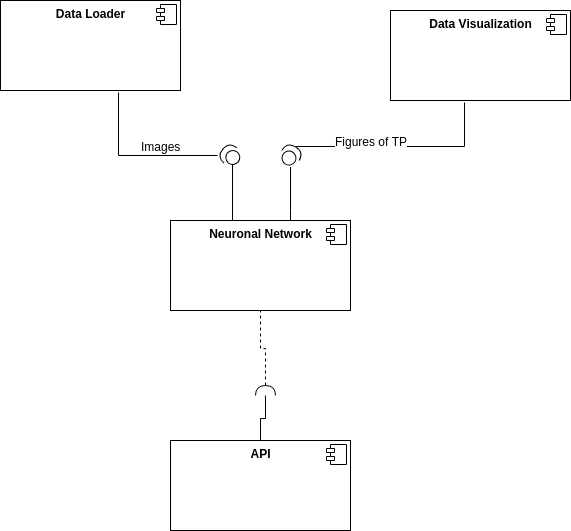
\includegraphics[width=0.8\textwidth]{./figures/component-uml}
\caption{Component UML of the system.}
\end{figure}

The system is based on 3 main components, the Data Loader whose main objective is to load the images from the trainnig and tests folders in an efficient way. The Data Visualization is the responsible of give the plots and figures of the trainning process to evaluate and monitor it. The Neuronal Network will train the model to predict the skin cancer images that we will use in the API component. 


\subsection{Use Cases UML}


\begin{figure}[H]
\centering
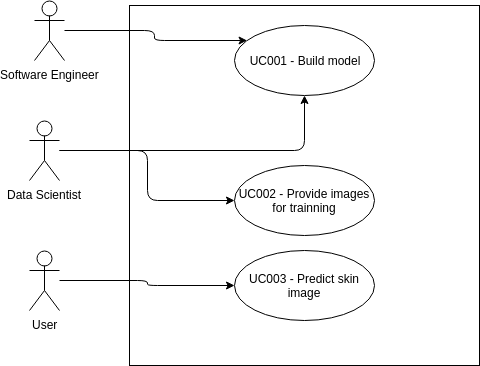
\includegraphics[width=0.8\textwidth]{./figures/use-case-uml}
\caption{Use Cases UML.}
\end{figure}

\subsubsection{Definition of the use cases}

\FloatBarrier
\begin{table*}[htb]
	\centering
	\begin{coolTable}{p{4cm}p{\textwidth-4.5cm}}{2}
{UC001: Build model}
	\textbf{Version}&1.0\\
	\textbf{Author}&Álvaro González Jiménez\\
	\textbf{Description}&The system must behave like in the following secuence diagram\\
	\textbf{Priority}&High \\
	\textbf{Status}&Done\\
	\textbf{Comments}& - \\	
	\end{coolTable}
	\caption{UC001: Build model}
\end{table*}
\FloatBarrier


\FloatBarrier
\begin{table*}[htb]
	\centering
	\begin{coolTable}{p{4cm}p{\textwidth-4.5cm}}{2}
{UC002: Provide images for trainning}
	\textbf{Version}&1.0\\
	\textbf{Author}&Álvaro González Jiménez\\
	\textbf{Description}&The system must provide an easy process to store the images for trainning and provide them to the neuronal network throught the Data Loader.\\
	\textbf{Priority}&High \\
	\textbf{Status}&Done\\
	\textbf{Comments}& - \\	
	\end{coolTable}
	\caption{UC002: Provide images for trainning}
\end{table*}
\FloatBarrier


\FloatBarrier
\begin{table*}[htb]
	\centering
	\begin{coolTable}{p{4cm}p{\textwidth-4.5cm}}{2}
{UC003: Predict skin image}
	\textbf{Version}&1.0\\
	\textbf{Author}&Álvaro González Jiménez\\
	\textbf{Description}&The system must behave like in the secuence diagram to predict a new image.\\
	\textbf{Priority}&High \\
	\textbf{Status}&Done\\
	\textbf{Comments}& - \\	
	\end{coolTable}
	\caption{UC003: Predict skin image}
\end{table*}
\FloatBarrier

\subsection{API definition}

In this subsection we are going to define the API that we will consume to predict the new images for the APP. 

The API only has a endpoint which is the responsible to receive the image from the APP, evaluate it with the trainned model and return the result throught a JSON.

We can think that the endpoint should use the GET attribute because we want to get some information about an image. However, it is not possible to send an image with the GET attribute so we must use the POST attribute for that. 

\begin{table*}[htb]
	\centering
	\begin{coolTable}{p{4cm}p{\textwidth-4.5cm}}{2}
{Endpoint 1 - Predict an skin image}
	\textbf{URI}&1.0\\
	\textbf{HTTP Attribute}&Álvaro González Jiménez\\
	\textbf{Content-Type}&Application/x-www-form-urlencoded\\
	\textbf{Input key}&"image"\\
	\textbf{Input key}&The image which we want to get the information about.\\	
	\textbf{Type of answer}&JSON\\
	\textbf{Example of anwer}&{"class": "melanoma", "probability": 0.823556}\\	
	\end{coolTable}
	\caption{Endpoint 1 - Predict an skin image}
\end{table*}

\subsection{APP Prototype}

As we have described in the previous section we are going to build an APP that consumes the services of the API, this is just a prototype for research porpouses. However, we can include more features to this APP and sell it as a product or SAAS.

The APP must work in the most important platforms, Android and IOs. Furthermore, we have to be able to take a picture from the camera or get it from the gallery. We need a simple APP so we will implement one screen with the input data and show the results on the same. 


\begin{figure}[H]
\centering
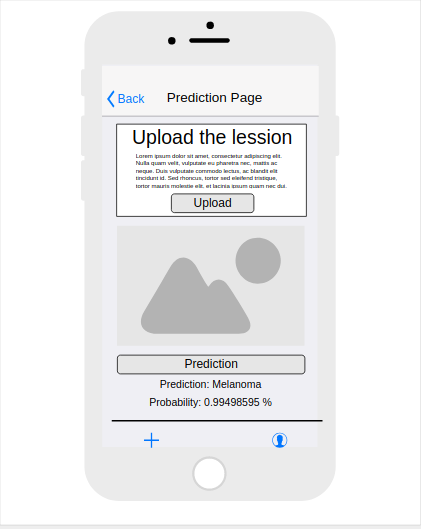
\includegraphics[width=0.8\textwidth]{./figures/Mockup}
\caption{Mockup of the APP.}
\end{figure}


\begin{figure}[H]
\centering
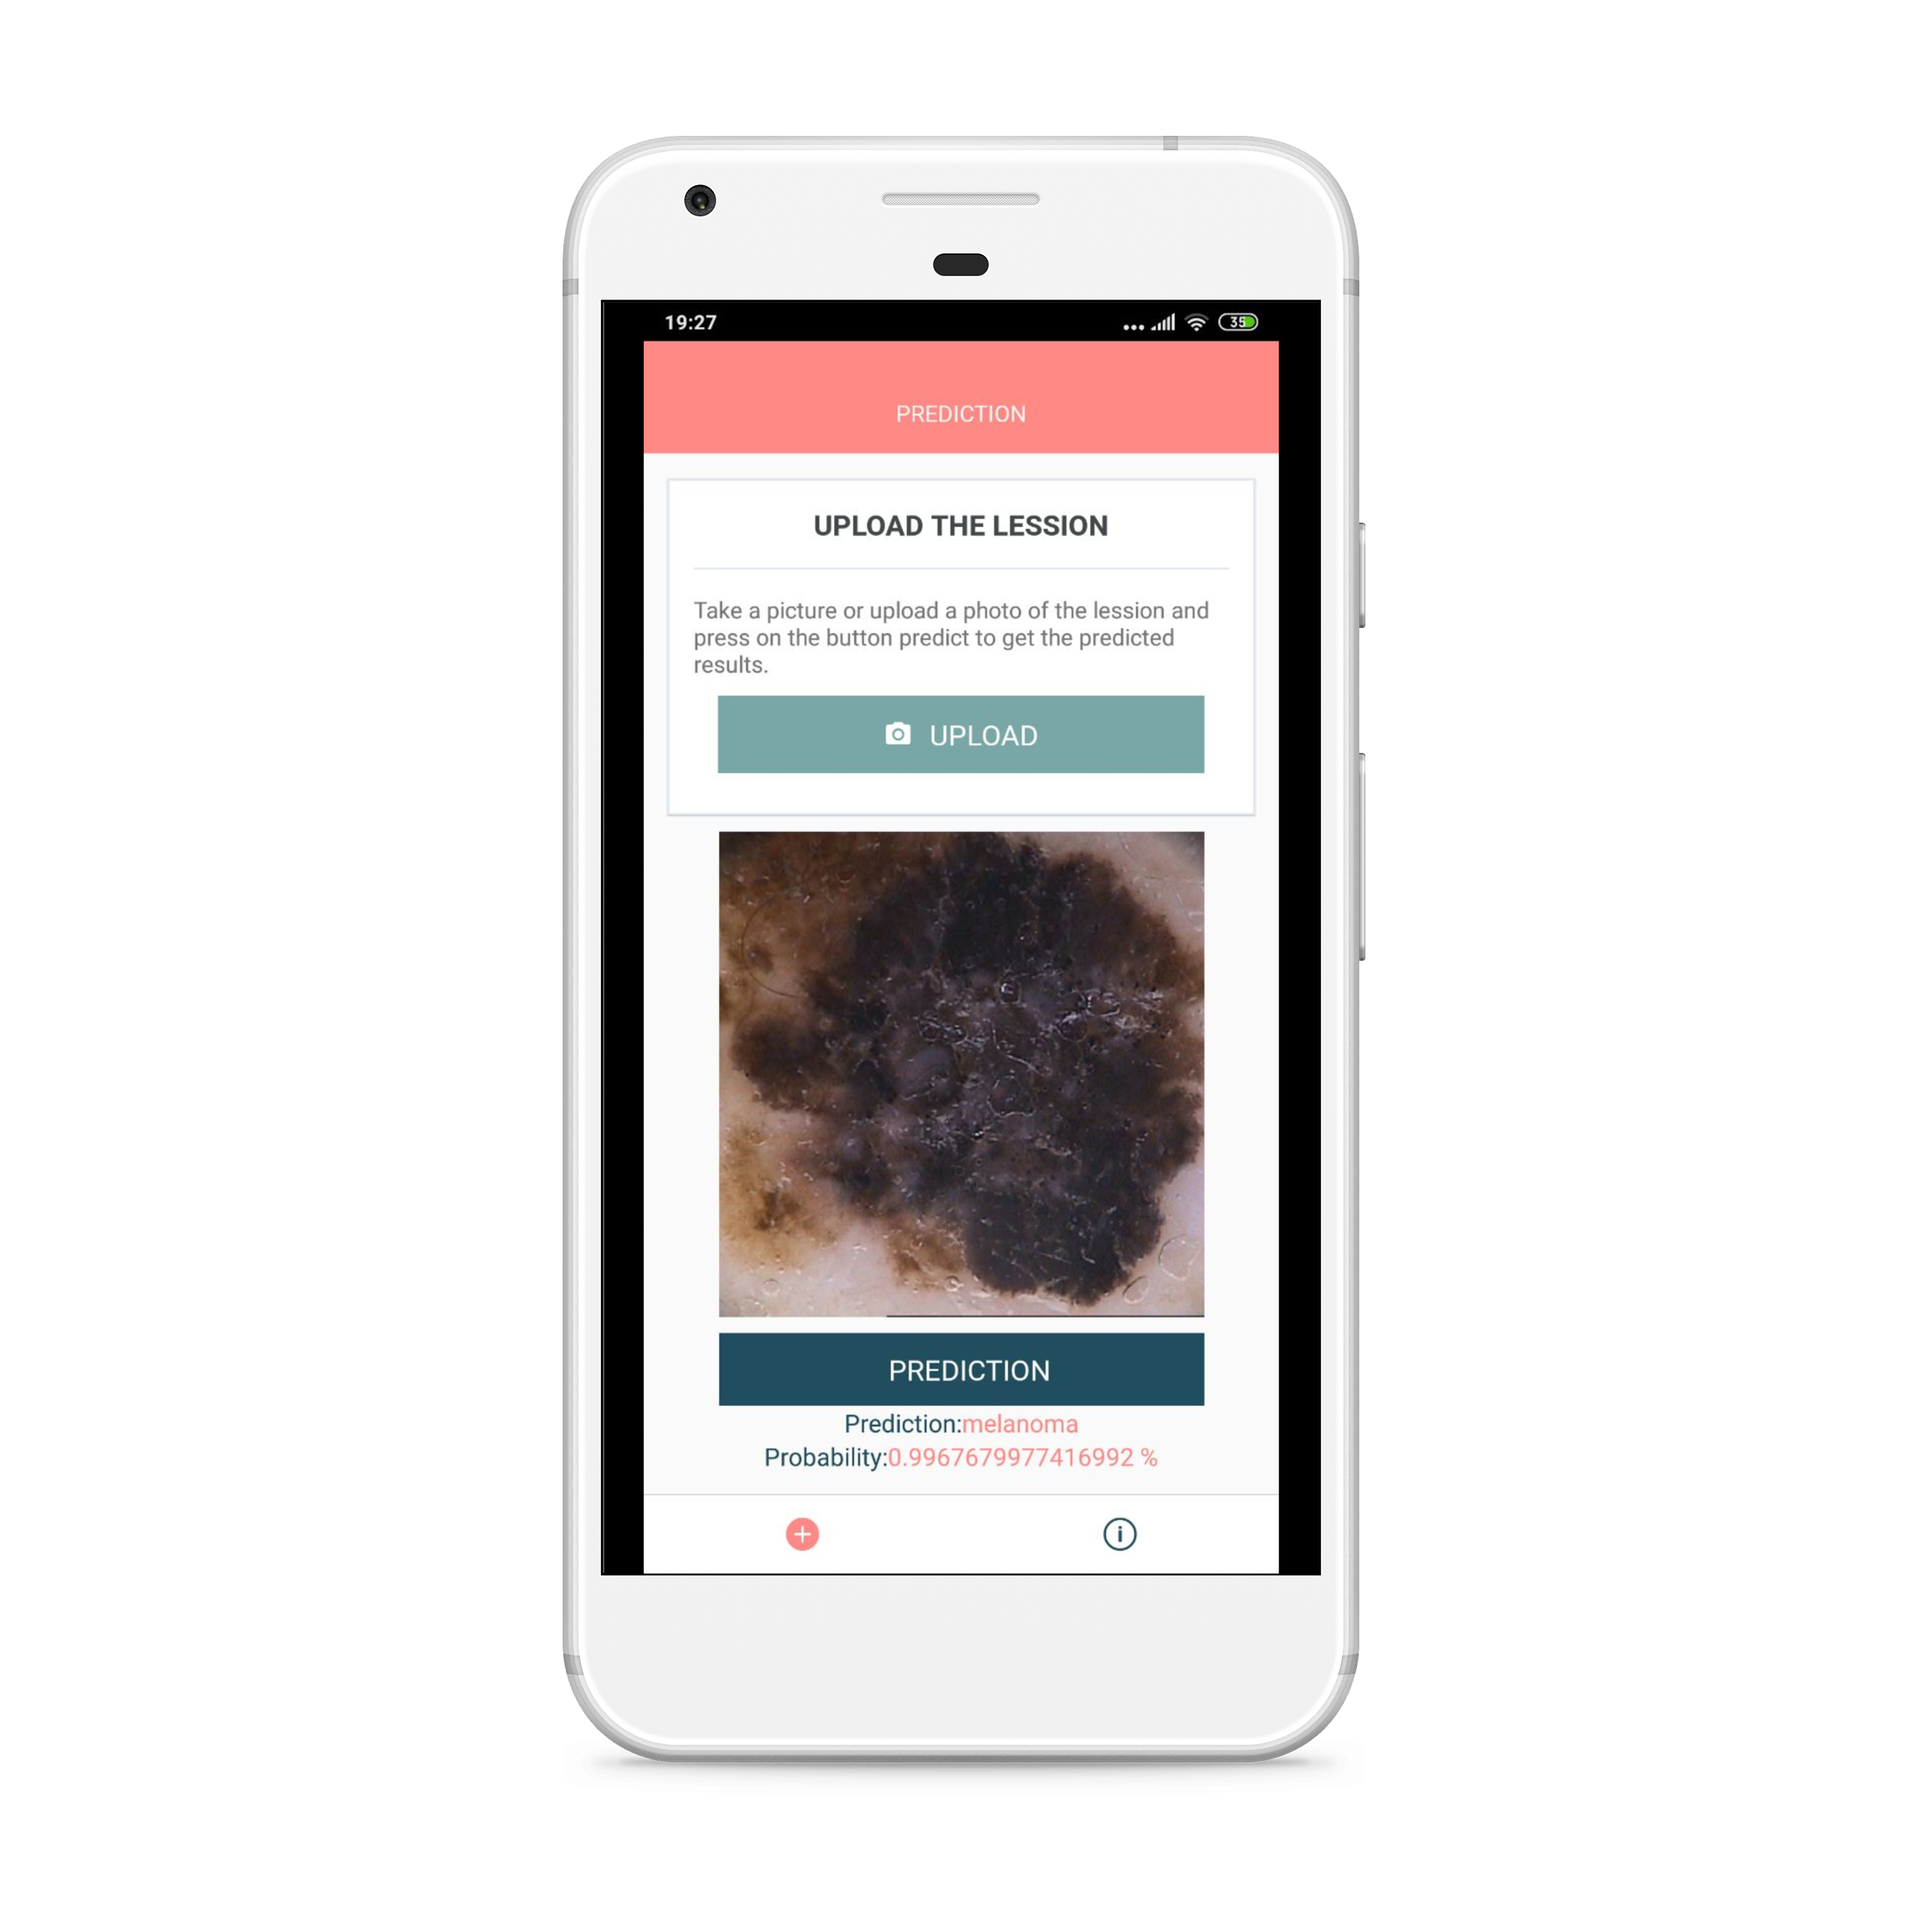
\includegraphics[width=1\textwidth]{./figures/mockup-android}
\caption{Final version of the APP.}
\end{figure}



\section{Plannification}

We are going to follow the structure of a 	classical AI projects wich contains the following steps:

\begin{enumerate}
\item Obtain the data 
\item Cleaning and preprocessing the data
\item Build a model
\item Evaluate it and tunning it to improve the results
\item Deploy the model or expose it in an API
\end{enumerate}

We will define the structure of the projet in the EDT (next section).

\subsection{Resources availables}

\subsubsection{Hardware and Software}

The hardware is one of the most important thing in an AI project, it will determine the time to get the results of the model. Nowdays GPUs provide a great deal of speed in calculus and mathematics operations. In our case we haven't got the machines with GPUs, but we can use one of the famous GPUs clouds (AWS, Google Cloud, Paperspace, Floydhub, etc). 

There are plenty of GPUs clouds services if we compare them the best between hardware and price is Paperspace \cite{gpu-cloud}. 

\FloatBarrier

\begin{table*}[htb]
	\centering
	\begin{coolTable}{p{4cm}p{\textwidth-4.5cm}}{2}
{Machine 1 - Laptop}
	\textbf{Model}& Lenovo G710\\
	\textbf{CPU}&Intel Core i7-4702MQ 2.2 GHz,\\
	\textbf{GPU}&NVIDIA GeForce 820m\\
	\textbf{RAM Memory}&8GB\\
	\textbf{OS}&Ubuntu 18.04\\	
	\end{coolTable}
	\caption{Machine 1 - Laptop}
\end{table*}


\begin{table*}[htb]
	\centering
	\begin{coolTable}{p{4cm}p{\textwidth-4.5cm}}{2}
{Machine 2 - Paperspace Server}
	\textbf{Model}& P5000\\
	\textbf{CPU}&Intel Xeon E5-2623 v4\\
	\textbf{GPU}&NVIDIA Quadro P5000 with 2560 CUDA cores.\\
	\textbf{RAM Memory}&30GB \\
	\textbf{OS}&Ubuntu 18.04\\	
	\textbf{Price}&0.78 \$/hour\\		
	\end{coolTable}
	\caption{Machine 2 - Paperspace Server}
\end{table*}

\FloatBarrier

The machine 1 will be used to read the articles, write the documentation and train the base model because it hasn't got the enought resources and power to train the entire dataset, it will take more than 1 week to train the dataset.  

The machine 2 will be used to train the models, modify them and get the best accuracy. The trainning time in this machine will take few hours.

The software that we will use in the machine 1 are:
\begin{enumerate}
\item Microsoft Office 360
\item Draw.io
\item TexMaker (Latex)
\item Python 3.5
\item Jupyter Notebook
\item Pytorch

\end{enumerate}

The software that we will use in the machine 2 are:
\begin{enumerate}
\item Python 3.5
\item Jupyter Notebook
\item Pytorch
\end{enumerate}



\subsubsection{People}

The only available person to make this project is myself cause this is a final degree project. My supervisor will guide me, give me advises to build a good project but she is not going to implement it. 

\FloatBarrier
\begin{table*}[htb]
	\centering
	\begin{coolTable}{p{4cm}p{\textwidth-4.5cm}}{2}
{Person 1 - Dr. Isabel Nepomuceno Chamorro}
	\textbf{Rol}&Supervisor\\
	\textbf{Organization}&Dpto. de Lenguaje y Sistemas Informaticos (LSI)	\\
	\textbf{Description}&Member of the LSI department, she will guide the student to
	build good project and review the documentation.\\
	\end{coolTable}
	\caption{People 1 - Dr. Isabel Nepomuceno Chamorro}
\end{table*}
\FloatBarrier


\FloatBarrier
\begin{table*}[htb]
	\centering
	\begin{coolTable}{p{4cm}p{\textwidth-4.5cm}}{2}
{Person 2 - Álvaro González Jiménez}
	\textbf{Rol}&Software Engineer\\
	\textbf{Organization}&Dpto. de Lenguaje y Sistemas Informaticos (LSI)	\\
	\textbf{Description}&	Software engineer student, he has the reponsability to implement the software, train the models, and write the documentation of the project.\\
	\end{coolTable}
	\caption{People 2 - Álvaro González Jiménez}
\end{table*}
\FloatBarrier


\subsection{Work Breakdown Structure}

\begin{figure}[H]
\centering
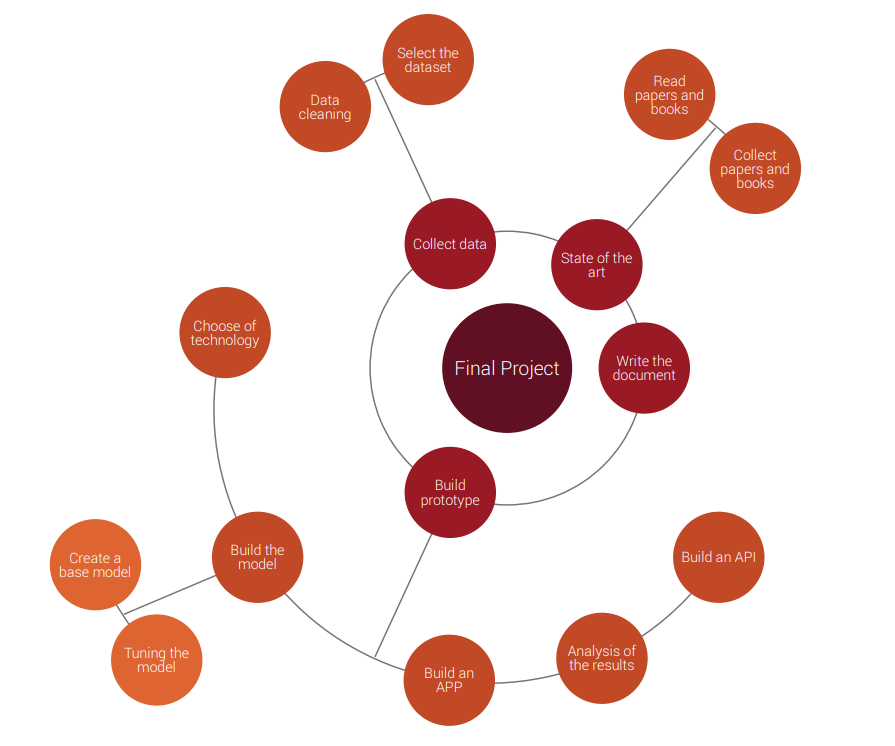
\includegraphics[width=1\textwidth]{./figures/edt}
\caption{Mind map of the project}
\end{figure}


\begin{figure}[H]
\centering
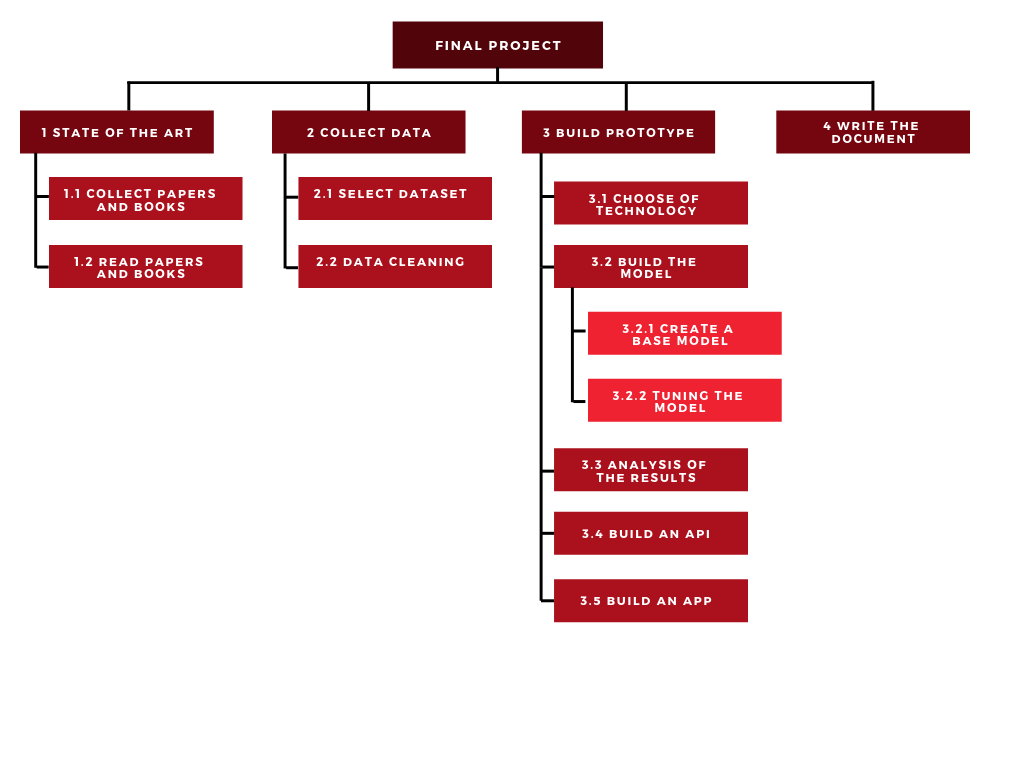
\includegraphics[width=1\textwidth]{./figures/wbs-project}
\caption{Work Breakdown Structure}
\end{figure}


\FloatBarrier
\begin{table*}[htb]
	\centering
	\begin{coolTable}{p{4cm}p{\textwidth-4.5cm}}{2}
{State of the art}
	\textbf{ID}&1\\
	\textbf{Description}&Research the current state of the art for DL\\
	\textbf{Duration}&60 hours\\
	\textbf{People}& Álvaro González Jiménez\\
	\textbf{Resources}& Machine 1\\
	\end{coolTable}
	\caption{WBS: 1. State of the art}
\end{table*}
\FloatBarrier

\FloatBarrier
\begin{table*}[htb]
	\centering
	\begin{coolTable}{p{4cm}p{\textwidth-4.5cm}}{2}
{Collect papers and books}
	\textbf{ID}&1.1\\		
	\textbf{Description}&Get available documentation for the state of the art\\
	\textbf{Duration}&20 hours\\
	\textbf{People}& Álvaro González Jiménez\\
	\textbf{Resources}& Machine 1\\
	\end{coolTable}
	\caption{WBS: 1.1 Collect papers and books}
\end{table*}
\FloatBarrier

\FloatBarrier
\begin{table*}[htb]
	\centering
	\begin{coolTable}{p{4cm}p{\textwidth-4.5cm}}{2}
{Read papers and books}
	\textbf{ID}&1.2\\		
	\textbf{Description}&Read, understand and learn the concepts of the documentation\\
	\textbf{Duration}&40 hours\\
	\textbf{People}& Álvaro González Jiménez\\
	\textbf{Resources}& Machine 1\\
	\end{coolTable}
	\caption{WBS: 1.2 Read papers and books}
\end{table*}
\FloatBarrier


\FloatBarrier
\begin{table*}[htb]
	\centering
	\begin{coolTable}{p{4cm}p{\textwidth-4.5cm}}{2}
{Collect data}
	\textbf{ID}&2\\		
	\textbf{Description}&Obtain the needed data to build the models\\
	\textbf{Duration}&10 hours\\
	\textbf{People}& Álvaro González Jiménez\\
	\textbf{Resources}& Machine 1 and Machine 2\\
	\end{coolTable}
	\caption{WBS: 2 Collect data}
\end{table*}
\FloatBarrier


\FloatBarrier
\begin{table*}[htb]
	\centering
	\begin{coolTable}{p{4cm}p{\textwidth-4.5cm}}{2}
{Select the dataset}
	\textbf{ID}&2.1\\		
	\textbf{Description}&Analyze and evaluate the obtained dataset in order to choose another one or improve it.\\
	\textbf{Duration}&2 hours\\
	\textbf{People}& Álvaro González Jiménez\\
	\textbf{Resources}& Machine 1 and Machine 2\\
	\end{coolTable}
	\caption{WBS: 2.1 Select the dataset}
\end{table*}
\FloatBarrier


\FloatBarrier
\begin{table*}[htb]
	\centering
	\begin{coolTable}{p{4cm}p{\textwidth-4.5cm}}{2}
{Data cleaning}
	\textbf{ID}&2.2\\		
	\textbf{Description}&Preprocesing the images and data augmentation\\
	\textbf{Duration}&8 hours\\
	\textbf{People}& Álvaro González Jiménez\\
	\textbf{Resources}& Machine 1 and Machine 2\\
	\end{coolTable}
	\caption{WBS: 2.1 Data cleaning}
\end{table*}
\FloatBarrier


\FloatBarrier
\begin{table*}[htb]
	\centering
	\begin{coolTable}{p{4cm}p{\textwidth-4.5cm}}{2}
{Build the prototype}
	\textbf{ID}&3\\		
	\textbf{Description}&Create the prototype to test the initial hypothesis\\
	\textbf{Duration}&250 hours\\
	\textbf{People}& Álvaro González Jiménez\\
	\textbf{Resources}& Machine 1 and Machine 2\\
	\end{coolTable}
	\caption{WBS: 3 Build the prototype}
\end{table*}
\FloatBarrier



\FloatBarrier
\begin{table*}[htb]
	\centering
	\begin{coolTable}{p{4cm}p{\textwidth-4.5cm}}{2}
{Choice of technology}
	\textbf{ID}&3.1\\		
	\textbf{Description}&Analysis of the current technologies, choose one and learning it to build the prototype.\\
	\textbf{Duration}&20 hours\\
	\textbf{People}& Álvaro González Jiménez\\
	\textbf{Resources}& Machine 1\\
	\end{coolTable}
	\caption{WBS: 3 Choice of technology}
\end{table*}
\FloatBarrier



\FloatBarrier
\begin{table*}[htb]
	\centering
	\begin{coolTable}{p{4cm}p{\textwidth-4.5cm}}{2}
{Build the model}
	\textbf{ID}&3.2\\		
	\textbf{Description}&Make the model which will classify the images \\
	\textbf{Duration}&100 hours\\
	\textbf{People}& Álvaro González Jiménez\\
	\textbf{Resources}& Machine 1 and Machine 2\\
	\end{coolTable}
	\caption{WBS: Build the model}
\end{table*}
\FloatBarrier


\FloatBarrier
\begin{table*}[htb]
	\centering
	\begin{coolTable}{p{4cm}p{\textwidth-4.5cm}}{2}
{Create a base model}
	\textbf{ID}&3.2.1\\		
	\textbf{Description}&Make an initial model that we will improve it to get better results.\\
	\textbf{Duration}&20 hours\\
	\textbf{People}&Álvaro González Jiménez\\
	\textbf{Resources}& Machine 1 and Machine 2\\
	\end{coolTable}
	\caption{WBS: Create a base model}
\end{table*}
\FloatBarrier


\FloatBarrier
\begin{table*}[htb]
	\centering
	\begin{coolTable}{p{4cm}p{\textwidth-4.5cm}}{2}
{Tuning the model}
	\textbf{ID}&3.2.2\\		
	\textbf{Description}&Try different inputs and train differents models to get the best model.\\
	\textbf{Duration}&80 hours\\
	\textbf{People}&Álvaro González Jiménez\\
	\textbf{Resources}& Machine 2\\
	\end{coolTable}
	\caption{WBS: Tuning the model}
\end{table*}
\FloatBarrier


\FloatBarrier
\begin{table*}[htb]
	\centering
	\begin{coolTable}{p{4cm}p{\textwidth-4.5cm}}{2}
{Analysis of the results}
	\textbf{ID}&3.3\\		
	\textbf{Description}&Get the results of the differents models, analyze base on the metrics that we decided and choose the best one.\\
	\textbf{Duration}&30 hours\\
	\textbf{People}&Álvaro González Jiménez
	and  Dr. Isabel Nepomuceno Chamorro\\
	\textbf{Resources}& Machine 1\\
	\end{coolTable}
	\caption{WBS: Analysis of the results}
\end{table*}
\FloatBarrier

\FloatBarrier
\begin{table*}[htb]
	\centering
	\begin{coolTable}{p{4cm}p{\textwidth-4.5cm}}{2}
{Build an API}
	\textbf{ID}&3.4\\		
	\textbf{Description}&Make an API to get skin images and predict the label.\\
	\textbf{Duration}&50 hours\\
	\textbf{People}&Álvaro González Jiménez\\
	\textbf{Resources}& Machine 1\\
	\end{coolTable}
	\caption{WBS: Build an API}
\end{table*}
\FloatBarrier


\FloatBarrier
\begin{table*}[htb]
	\centering
	\begin{coolTable}{p{4cm}p{\textwidth-4.5cm}}{2}
{Build an APP}
	\textbf{ID}&3.5\\		
	\textbf{Description}&Make a small APP wich will take pictures or send pictures of the skin lession to the API in order to get the information about the lession.\\
	\textbf{Duration}&50 hours\\
	\textbf{People}&Álvaro González Jiménez\\
	\textbf{Resources}& Machine 1\\
	\end{coolTable}
	\caption{WBS: Build an APP}
\end{table*}
\FloatBarrier


\FloatBarrier
\begin{table*}[htb]
	\centering
	\begin{coolTable}{p{4cm}p{\textwidth-4.5cm}}{2}
{Write the document}
	\textbf{ID}&4\\		
	\textbf{Description}&Write all the documentation of the project in English and review it.\\
	\textbf{Duration}&50 hours\\
	\textbf{People}&Álvaro González Jiménez and 
 Dr. Isabel Nepomuceno Chamorro\\
	\textbf{Resources}& Machine 1\\
	\end{coolTable}
	\caption{WBS: Write the document}
\end{table*}
\FloatBarrier






\section{Costs}  

In the people table we can see there are two types of participants in the project. Data scientist and project supervisors in order to estimate the cost of the project we will count the hour of each type employee and multiply it by the cost per hour associated to each type of employee.

It is worth mentioning that this is a final degree project, even if the author takes on the role of data scientist we are talking about a person without experience, knowledge and non graduated so the salary will be affected.

In case of the supervisor of the project, due to the fact that she is a PhD teacher with a great deal of experience her salary will be higher.


\FloatBarrier
\begin{table*}[htb]
	\centering
	\begin{coolTable}{p{4cm}p{\textwidth-4.5cm}}{2}
{People salary}
	\textbf{Álvaro González}&18.000 €/per year\\		
	\textbf{Isabel Nepomuceno}&30.000 €/per year\\
	\end{coolTable}
	\caption{People salary}
\end{table*}
\FloatBarrier

Assuming a total of 1722 hours per year we will get the nexts results.

\[ 18000 / 1722 = 10,45 eur/hour \]
\[ 30000 / 1722 = 17,42 eur/hour \]


\begin{table}[H]
	\centering    
    \begin{tabular}{|l|l|c|}
    \hline
    Person            & Estimate hours & Cost    \\ \hline
    Alvaro Gonzalez   & 370            & 3866,5€ \\ \hline
    Isabel Nepomuceno & 20             & 348,4€  \\ \hline
    Total             & 390            & 4214,9€  \\ \hline
    \end{tabular}
\end{table}

Secondly, we will calculate the amortization of hardware equipment in 4 years, which will give us an annual amortization quota. This annual amortization cost will be multiplied by the time of use of these equipment during the project, which will result in the cost associated with the project of each of the hardware equipment.

In the case of the second machine (server) hasn't got any amortization because we are not the owners of this hardware, we are going to pay as long as we use it.

The cost of the first machine is 900€ (C). We know that the porcentage that we can use for the amortization is 10\% for a maximum of 4 years.

\[ M = 900 eur * 0.1 * 4 = 360 eur \]

\[ B = C - M = 900 eur - 360 eur = 540 eur\]

\[Annual repayment = 540 eur / 4 years = 135€/year\]

The project will be done in 9 months so the cost associated is:

\[Annual repayment = 135 eur * 0.75 year = 101,25 eur\]

The cost of using the second machine is:
\[0,78€/hour * 100 hours = 78 eur\]

\newpage
In this section we will make the sum of all the costs associated with the project, which are mainly personnel costs and hardware costs. Knowing that the personnel costs amount to 4214,9€ and the hardware costs, to 179,25€. We have that the total cost of the project is 4214,9€ + 179,25€ = 4.394,45€. 
\FloatBarrier
\begin{table*}[htb]
	\centering
	\begin{coolTable}{p{4cm}p{\textwidth-4.5cm}}{2}
{Summary of the cost of the project}
	\textbf{People salary}&4214,9 €\\		
	\textbf{Machine 1}&101,25 €\\
	\textbf{Machine 2}&78 €\\
	\textbf{Total}&4.394,15 €\\
	\end{coolTable}
	\caption{Summary of the cost of the project}
\end{table*}
\FloatBarrier


\chapter{Evaluation of the Models}

\begin{abstract}
In this chapter we are going to detail the results that we have obtained in the different models comparing it with the metrics that we had defined in the evaluation section of the model.
\end{abstract}


\section{Results}

At the beginning, in the section on transfer of learning, the models that we were going to use were defined and their subsequent result was measured. The models are distinguished by the complexity of the architecture, the hyperparameters that have been used and the learning period. 

The first model is the simplest of the three, using a resnet architecture with a total of 18 layers and 11 training periods. Thanks to these parameters the time needed to train the model has been approximately 4 hours.
The accuracy of this model is 75\%, you can see in the following image as the model has evolved over the years.


\begin{figure}[H]
\centering
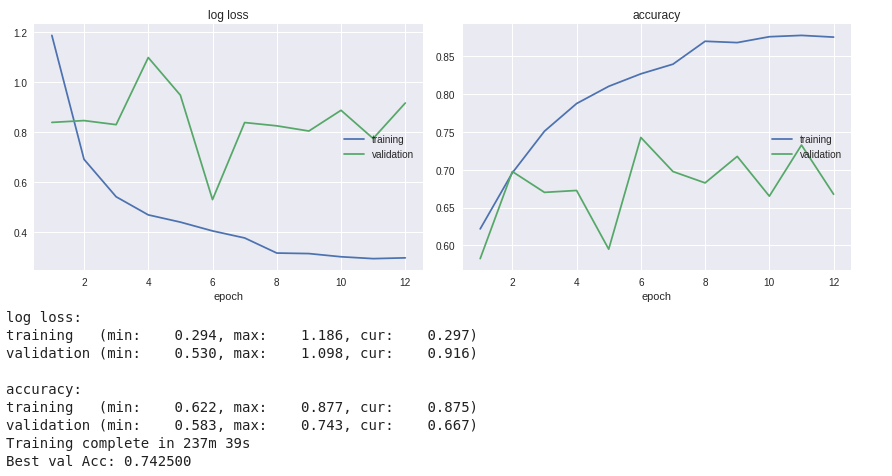
\includegraphics[width=0.8\textwidth]{./figures/resnet-18}
\caption{Training of ResNet-18.}
\end{figure}


The second model is an evolution of the previous one, we used the same architecture but with a higher number of layers (50) and a total of 21 epochs instead of 11. The good thing about this architecture is that you can increase the number of layers as we want and we will see a greater precision. However, there is also an over-training called overfitting in the training dataset. Also due to the complexity of the same and the number of epochs that have been established has needed a total of 7 hours to complete the training. The accuracy of this model is 88\% being the highest of the three.


\begin{figure}[H]
\centering
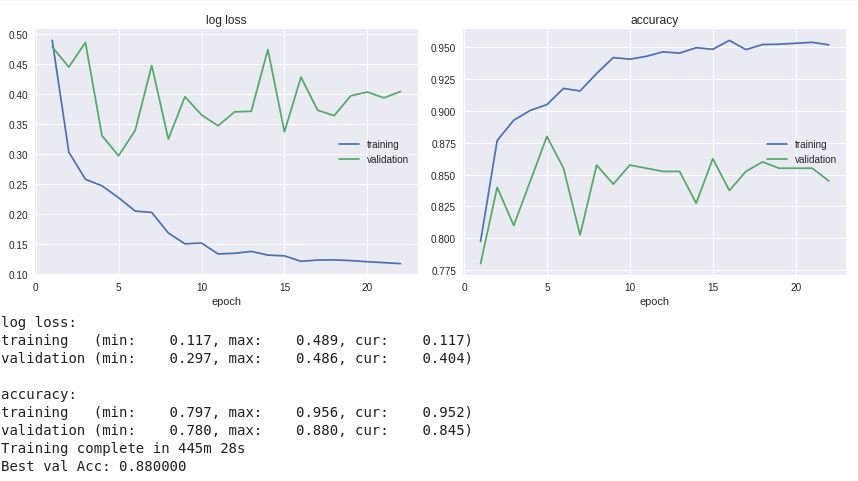
\includegraphics[width=0.8\textwidth]{./figures/resnet-50}
\caption{Training of ResNet-50.}
\end{figure}

The last model the architecture used is a ResNet alteration called DenseNet in which overtraining in small data sets is reduced and your training is more efficient than in the ResNet architecture. Although in our case has not been so, we have needed the same number of hours 7 hours and observe a greater overfitting using this architecture and parameters. The accuracy of this model has been 85\% higher than ResNet-18 but lower than ResNet-50.


\begin{figure}[H]
\centering
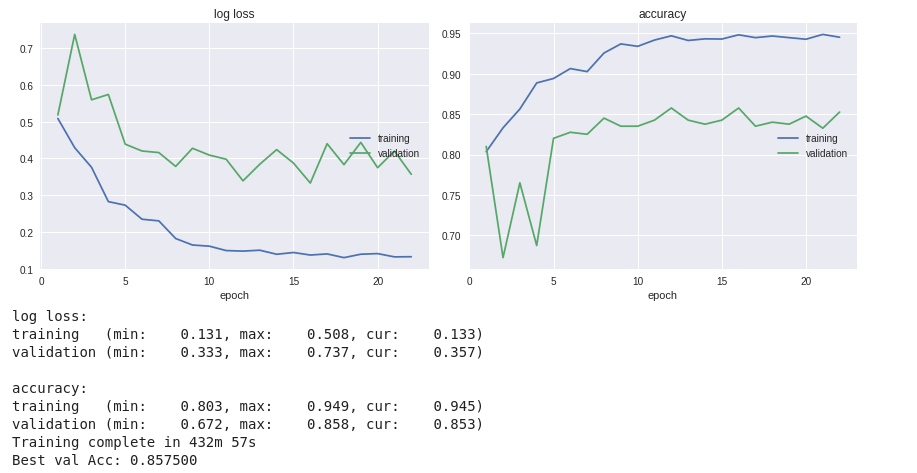
\includegraphics[width=0.8\textwidth]{./figures/densenet-121}
\caption{Training of Densenet-121.}
\end{figure}


In conclusion, the model we have selected has been the second (Resnet-50) due to the precision it gives us. In the following section we are going to calculate the sensitivity, the specificity and the area under the ROC curve.


\subsection{Obtaining the Confusion Matrix}

\begin{figure}[H]
\centering
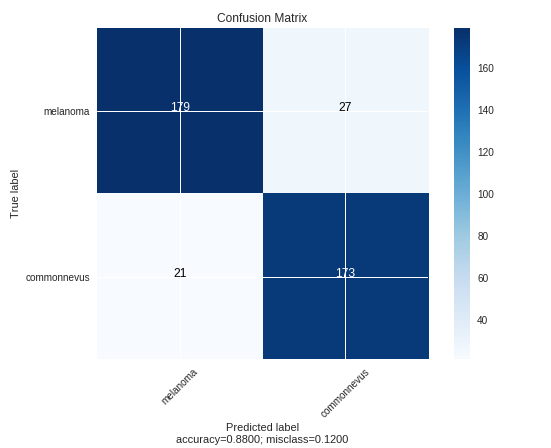
\includegraphics[width=1\textwidth]{./figures/confusion-matrix-resnet50}
\caption{Confusion matrix of the model.}
\end{figure}

\begin{figure}[H]
\centering
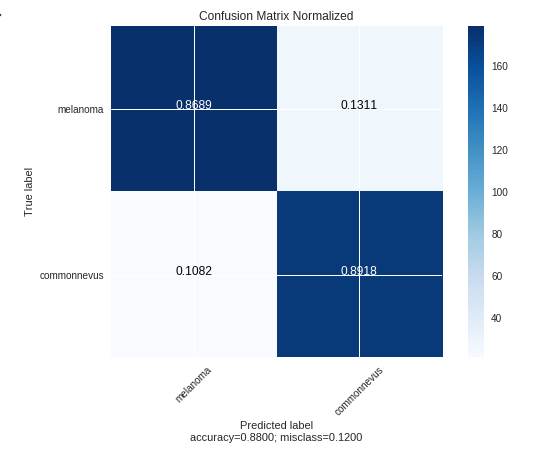
\includegraphics[width=1\textwidth]{./figures/confusion-matrix-normalized-resnet50}
\caption{Confusion matrix normalized of the model.}
\end{figure}

The confusion matrix has been obtained on the test data set because if we use the training data set the result obtained and the metrics would be erroneous. From the confusion matrix we will compute the other metrics

\begin{enumerate}
\item TP = 179
\item FP = 27
\item TN = 173
\item FN = 21
\end{enumerate}

Sensitivity will tell us which of the patients who really have skin cancer have been diagnosed with skin cancer
\[ Sensitive = TP/(TP+FN) = 179 / (179+21) = 0,895 \]

Specificity measures the number of patients who do not have skin cancer have been categorized as having no skin cancer.
\[ Specificity  = TN/(TN+FP) = 173 / (173+27) = 0,865 \]

PVP will measure the proportions of positive and negative results in statistics and diagnostic tests that are true positive.The ideal value of the PPV, with a perfect test, is 1 (100\%)
\[ PVP = TP/(TP+FP) = 179 / (179+27) = 0,868 \]

NPV will measure the proportions of positive and negative results in statistics and diagnostic tests that are true negative. The ideal value of the NPV, with a perfect test, is 1 (100\%)
\[ NPV = TN/(TN+FN) = 173 / (173+21) = 0,892 \]

In the metrics it can be seen that the classifier is quite homogeneous, and things don't happen that are difficult to interpret. The classifier, as can be seen in the confusion matrix, has a fairly stable level of success in both classes, which indicates that it has correctly generalized the detection of cancer in the images. in short, the classifier has behaved very well compared to this set of images with respect to other classifiers and techniques. 

Even knowing that medical images are complicated to deal with, the classifier has been able to generalize the details that separate a image of a patient who suffers from skin cancer of another patient who does not suffer from it, thus achieving predict accurately in most cases.
